\section{Introducción}

\subsection{Contexto y justificación del trabajo}

Un campo de distancia con signo (\textit{Signed Distance Field}, SDF) es una representación espacial que asigna a cada punto del espacio la distancia mínima hasta la superficie geométrica más cercana, utilizando el signo para distinguir el interior del exterior cuando la geometría admite esa clasificación. Esta formulación permite consultar de manera directa tanto la proximidad a una frontera como la dirección hacia ella a través del gradiente del campo. Gracias a estas propiedades, los SDF se utilizan en ámbitos diversos de la computación espacial más allá de la síntesis de imagen: en simulación física y detección de colisiones, donde los valores negativos cuantifican la profundidad de penetración entre cuerpos y el gradiente define la normal de contacto \cite{ericson2004, macklin2020}; y en robótica y visión por computador, donde permiten reconstruir el entorno a partir de sensores de profundidad para planificar trayectorias libres de obstáculos o simular la interacción física con objetos escaneados \cite{oleynikova2017}.

Dentro del desarrollo de videojuegos y la computación gráfica interactiva, además de su utilidad en motores de física, los SDF destacan como estructura de aceleración para el trazado de rayos por software mediante el algoritmo de \textit{sphere tracing} \cite{hart1996}, que adapta la longitud de los pasos de un rayo según la distancia segura a la superficie. Una de las aplicaciones más exigentes de este enfoque es la iluminación global en tiempo real, que plantea un compromiso constante entre calidad visual y coste de cálculo. Además de la luz que llega directamente desde una fuente hasta una superficie, la iluminación global considera las contribuciones indirectas producidas por las reflexiones sobre otras superficies de la escena, descritas por la ecuación de renderizado \cite{kajiya1986}. Estas interacciones permiten representar fenómenos como la transferencia de color entre objetos próximos, conocida como \textit{color bleeding} (Figura~\ref{fig:color_bleeding}).

\begin{figure}[htbp]
  \centering
  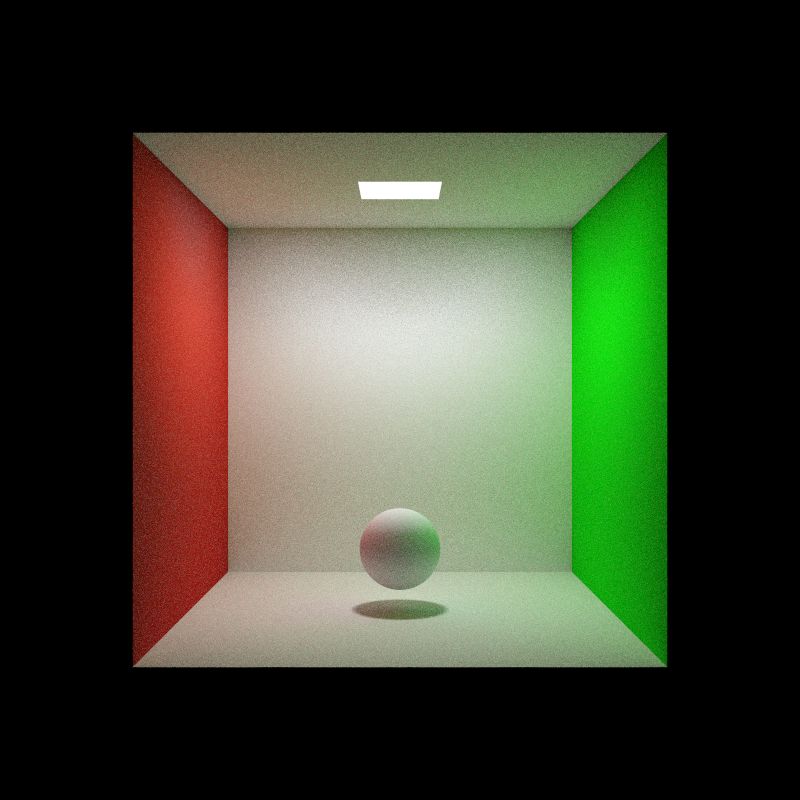
\includegraphics[width=0.78\textwidth]{docs/assets/screenshot_20261011_164754.png}
  \caption{Ejemplo de iluminación global con transferencia de color (\textit{color bleeding}): la luz rebota en el suelo e ilumina la parte inferior de la esfera; la luz reflejada en las paredes modula el sombreado de la esfera con el color de cada pared.}
  \label{fig:color_bleeding}
\end{figure}

En este contexto, sistemas de iluminación modernos como Lumen, de Unreal Engine 5 \cite{wright2022}, constituyen una referencia del empleo de campos de distancia discretizados para realizar consultas espaciales sin depender exclusivamente de hardware dedicado de trazado de rayos. No obstante, en una representación volumétrica discretizada, la precisión del campo y los errores de aproximación pueden afectar a las consultas espaciales y producir artefactos visuales, por lo que su comportamiento debe evaluarse. El presente trabajo se centrará en la generación de dichos campos en GPU y en una demostración acotada de su uso en iluminación global, sin intentar reproducir un sistema de iluminación de la complejidad de Lumen.

La generación del volumen de distancias es uno de los problemas centrales que plantea el uso de SDF en todos estos dominios. Cuando se parte de mallas poligonales, el cálculo exacto de distancias entre los puntos de una cuadrícula tridimensional y los triángulos de una malla puede requerir un número elevado de evaluaciones, cuyo coste crece con la resolución del volumen y la complejidad de la geometría. Aunque el precálculo resulta suficiente para entornos estáticos, reducir el tiempo de generación permitiría explorar actualizaciones más frecuentes y ampliar sus condiciones de uso.

La motivación práctica del proyecto parte de un límite concreto de un prototipo previo del autor: el visor existente utiliza únicamente primitivas SDF analíticas. Para trabajar con geometría poligonal arbitraria, se propone sustituir estas primitivas por texturas tridimensionales que almacenen el campo de distancias generado en GPU. Esta transición proporciona un banco de pruebas controlado para estudiar la construcción del volumen y observar cómo sus imprecisiones afectan al resultado visual.

El trabajo comparará un método base de cálculo de distancias punto-triángulo en GPU con una alternativa que combine la captura de datos de superficie mediante rasterización y la propagación espacial mediante \textit{Jump Flooding} (JFA) \cite{rong2006}. Al partir de datos superficiales proyectados en lugar de evaluar cada triángulo de la malla desde cada vóxel, esta segunda aproximación no solo busca desacoplar la fase de propagación de la complejidad poligonal en gráficos, sino que también guarda paralelismo con la construcción de campos de distancia a partir de capturas parciales o sensores de profundidad en simulación física y robótica. La pregunta que orienta la evaluación es qué compromiso ofrece esta alternativa entre tiempo de generación, consumo de memoria y error de distancia respecto al método de referencia.

El producto será un prototipo técnico de generación y evaluación de SDF, acompañado de un visor interactivo, dentro del área de programación gráfica y motores de videojuegos. En el visor se podrá cargar una escena de prueba, seleccionar el campo generado por cada método, inspeccionar cortes del volumen y observar su utilización en la iluminación. La generación de los campos y su comparación constituirán el núcleo del trabajo; el visor actuará como herramienta de demostración y análisis.

\subsection{Objetivos del trabajo}

\subsubsection{Objetivo general}

Diseñar, implementar y evaluar dos métodos de generación de campos de distancia con signo en GPU a partir de mallas poligonales, comparando una alternativa basada en rasterización y propagación espacial con un método de referencia, y analizando su tiempo de generación, consumo de memoria y precisión mediante pruebas numéricas y un visor interactivo de iluminación.

\subsubsection{Objetivos específicos}

\textbf{OE1. Adaptar el visor de partida.} Integrar el prototipo previo del autor en una aplicación modular en C++ con OpenGL 4.6 y SDL3, con controles de cámara, iluminación e interfaz, para disponer de un entorno de pruebas durante el desarrollo.

\textbf{OE2. Incorporar el muestreo de campos volumétricos.} Sustituir las primitivas SDF analíticas por el muestreo de texturas tridimensionales de distancia, adaptando el \textit{ray marching} para representar iluminación indirecta difusa de un rebote, oclusión ambiental y sombras suaves. El sombreado utilizará también la información de superficie necesaria.

\textbf{OE3. Implementar y comprobar el método de referencia.} Desarrollar un generador de distancias volumétricas en GPU mediante \textit{compute shaders}. Antes de utilizar sus resultados como referencia, comprobar su funcionamiento con geometrías de control cuyas distancias sean conocidas.

\textbf{OE4. Implementar la alternativa de generación rápida.} Diseñar y desarrollar un método que combine la extracción de datos de superficie mediante rasterización de un G-Buffer con la propagación mediante JFA en tres dimensiones. Se estudiarán la cobertura de la captura, el comportamiento de la propagación y el procedimiento de determinación del signo.

\textbf{OE5. Facilitar la inspección y comparación de los campos.} Incorporar un selector entre los volúmenes generados por ambos métodos y modos de visualización para examinar cortes del volumen y componentes de iluminación. La visualización adicional de vóxeles tendrá menor prioridad que estas herramientas.

\textbf{OE6. Ejecutar la evaluación experimental.} Diseñar y realizar pruebas sobre modelos geométricos de control y las escenas seleccionadas para comparar el tiempo de generación en milisegundos, el consumo de memoria de vídeo y el error de distancia de la alternativa respecto al método base. Las condiciones de comparación y el procedimiento de medición se concretarán durante la fase de diseño.

\subsubsection{Delimitación del alcance}

El trabajo se centrará en dos procedimientos de generación de SDF en GPU: un método de referencia y una alternativa basada en rasterización y JFA. No se plantea desarrollar un generador universal para cualquier tipo de malla ni un motor gráfico de propósito general.

Durante la fase de especificación y diseño se definirán las condiciones de entrada de las mallas, el procedimiento de obtención del signo, la captura de datos de superficie y el protocolo experimental. La selección final de las versiones de Cornell Box y Crytek Sponza dependerá de su adecuación a estas condiciones. Los modelos geométricos de control permitirán comprobar el funcionamiento antes de abordar escenas de mayor complejidad.

El rendimiento del visor se analizará por separado del tiempo de generación del campo. La navegación y la visualización deberán permitir examinar los resultados de forma interactiva, pero no se establece como requisito inicial reconstruir todo el volumen en cada fotograma.

Ante una reducción de alcance, se conservarán los dos generadores, su comprobación numérica, la comparación experimental y una demostración básica de iluminación indirecta difusa de un rebote. La inspección por cortes tendrá prioridad sobre la visualización de vóxeles. También podrán reducirse los controles secundarios de la interfaz y los refinamientos visuales, sin sustituir con ellos el trabajo de evaluación.

\subsection{Impacto en sostenibilidad, ético-social y de diversidad}

\subsubsection{Impacto en sostenibilidad}

El proyecto estudiará el uso de recursos computacionales mediante la comparación del tiempo y la memoria necesarios para generar campos de distancia en GPU. Los resultados permitirán identificar en qué condiciones una aproximación basada en propagación resulta ventajosa y qué pérdida de precisión puede introducir.

La implementación se planteará sin depender de extensiones específicas de trazado de rayos acelerado por hardware. No obstante, seguirá requiriendo una GPU compatible con las tecnologías seleccionadas.

El trabajo no incluirá mediciones de consumo energético ni de emisiones. Por tanto, una posible mejora del tiempo de ejecución o del uso de memoria no se presentará como una reducción demostrada del impacto ambiental.

\subsubsection{Impacto ético-social}

Se prevé publicar el código y la documentación para facilitar el estudio de los métodos y la reproducción de las pruebas. La documentación describirá los requisitos, las condiciones de reutilización y las limitaciones observadas.

Se mantendrá la atribución de las bibliotecas, modelos y fuentes utilizadas, así como una declaración del uso de asistentes de inteligencia artificial. La utilidad del proyecto para estudiantes y desarrolladores se considerará una contribución potencial, sin atribuirle una reducción demostrada de los costes de producción.

\subsubsection{Impacto en diversidad}

El proyecto no contempla recopilar datos demográficos ni realizar estudios con usuarios. Las medidas relacionadas con la diversidad se orientarán a facilitar el acceso al conocimiento mediante una documentación clara y una descripción de los requisitos técnicos.

La necesidad de disponer de una GPU compatible puede limitar el acceso al prototipo. Por ello, no se dará por supuesta su ejecución adecuada en equipos de prestaciones reducidas.

\subsection{Enfoque y método seguido}

El proyecto combinará un marco de investigación, un método de desarrollo del software y un sistema de seguimiento del trabajo.

\subsubsection{Marco de investigación}

Se utilizará la metodología de investigación en ciencias del diseño, \textit{Design Science Research Methodology} (DSRM), propuesta por Peffers et al. \cite{peffers2007}. Este marco organiza el trabajo alrededor de la construcción y evaluación de un artefacto tecnológico.

En este proyecto, el artefacto principal estará formado por los métodos de generación de campos de distancia en GPU. El visor servirá para demostrar su uso y examinar las consecuencias visuales de los campos obtenidos.

El proceso abarcará la identificación del problema, la definición de objetivos, el diseño y desarrollo, la demostración, la evaluación y la comunicación de resultados. La comparación experimental permitirá contrastar los métodos sin presuponer que la alternativa basada en JFA será superior en todas las métricas o escenas.

\subsubsection{Metodología de producción del software}

El desarrollo seguirá un enfoque incremental e iterativo basado en prototipos. Se adaptará primero el visor existente y se incorporará después el muestreo de texturas tridimensionales. Para esta integración inicial se utilizarán volúmenes de prueba, sin esperar a que los generadores a partir de mallas estén terminados.

A continuación, se incorporarán el método base, la alternativa JFA y los modos de inspección. Cada incremento se comprobará con casos reducidos antes de pasar a escenas de mayor complejidad.

Las decisiones de diseño y los problemas encontrados se documentarán durante la implementación. La memoria se redactará de forma progresiva, en lugar de concentrar toda la documentación al final del proyecto.

\subsubsection{Gestión del proyecto}

El seguimiento se realizará mediante un tablero Personal Kanban, con tareas vinculadas a los objetivos y a los hitos de entrega. Se revisará semanalmente el avance para detectar bloqueos, actualizar prioridades y registrar las desviaciones respecto a la planificación.

Git se utilizará para el control de versiones y la trazabilidad de los cambios, siguiendo la convención \textit{Conventional Commits}. Las revisiones con el tutor permitirán contrastar el alcance y orientar las decisiones que afecten a la viabilidad del trabajo.

\subsubsection{Distribución del trabajo entre entregas}

\textbf{PEC 1. Definición y planificación.} Se concretarán el problema, la motivación, los objetivos, el alcance y la planificación inicial. Esta entrega no incluirá nueva implementación del proyecto.

\textbf{PEC 2. Estado del arte, materiales y métodos y entorno de validación.} Se desarrollarán el capítulo 2 (estado del arte e hipótesis) y el capítulo 3 (estrategia de desarrollo, herramientas, protocolo experimental y entorno de pruebas). En el plano práctico, se consolidará y verificará el visor interactivo con filtrado SVGF (OE1) y se integrará el muestreo de texturas 3D mediante volúmenes de control generados por un \textit{compute shader} preliminar (avance de OE2), despejando los riesgos de integración antes de abordar la geometría poligonal.

\textbf{PEC 3. Diseño e implementación de generadores volumétricos a partir de mallas.} Se redactará el capítulo 4 (diseño y arquitectura) y se implementarán la carga y empaquetado de mallas en \textit{buffers} SSBO, el generador base de referencia punto-triángulo (OE3), el generador alternativo basado en captura de superficie y propagación JFA 3D (OE4) y el inspector de cortes bidimensionales (OE5). Se realizarán las primeras comprobaciones numéricas y mediciones comparativas.

\textbf{PEC 4. Evaluación y cierre.} Se completará la batería experimental, se analizarán los resultados y se redactarán las conclusiones. También se consolidará la memoria y se preparará la presentación y defensa en vídeo.

\subsection{Planificación del trabajo}

\subsubsection{Recursos necesarios}

\textbf{Hardware.} Se prevé utilizar una estación de trabajo con procesador multinúcleo x86-64, al menos 16 GB de memoria RAM y una tarjeta gráfica dedicada compatible con OpenGL 4.6, \textit{compute shaders} y texturas tridimensionales con acceso mediante \textit{shader image load/store}. Las resoluciones de trabajo se ajustarán a la memoria disponible y a los resultados de las pruebas.

\textbf{Software y entorno de desarrollo.} Se utilizará GNU/Linux, un compilador compatible con C++20 ---GCC o Clang---, CMake 3.20 o superior y Visual Studio Code. RenderDoc y las herramientas de monitorización de GPU servirán para inspeccionar recursos y analizar el comportamiento de la aplicación.

\textbf{Bibliotecas.} La aplicación utilizará SDL3, GLM, Assimp y Dear ImGui para la gestión de ventanas y entrada, las operaciones matemáticas, la importación de mallas y la interfaz.

\textbf{Modelos de prueba.} Se emplearán geometrías de control y las versiones seleccionadas de Cornell Box y Crytek Sponza, en formatos compatibles con el importador, como OBJ o glTF.

\subsubsection{Dedicación y seguimiento}

La planificación se elaborará a partir de una dedicación estimada de \textbf{20 horas semanales} (correspondiente a los 12 créditos ECTS de la asignatura, con un total estimado de 300 horas distribuidas a lo largo del semestre), que incluirá investigación, desarrollo, pruebas, documentación y revisión de las entregas.

La implementación principal se concentrará en el periodo correspondiente a la PEC 3. La documentación se mantendrá durante todas las fases, y la preparación del procedimiento de medición deberá quedar avanzada antes de comenzar la batería experimental final.

La disponibilidad durante el periodo final se tendrá en cuenta al concretar la dedicación. La entrega final de la PEC 4 se realizará el 23 de diciembre de 2026, concluyendo el trabajo antes del receso navideño. Si fuera necesario resolver incidencias durante la recta final, se ajustará el número de configuraciones experimentales secundarias, preservando la validez de la comparación principal entre los dos métodos.

El seguimiento semanal permitirá contrastar el trabajo realizado con el previsto y justificar las modificaciones del calendario.

\subsubsection{Hitos por PEC}

\textbf{PEC 1 --- 11/10/2026: definición del proyecto e introducción.} Se completarán la ficha del trabajo y el capítulo 1 de la memoria, con la justificación, los objetivos, el impacto, la metodología y la planificación. También se organizarán el repositorio y la documentación inicial.

\textbf{PEC 2 --- 08/11/2026: estado del arte, materiales y métodos y consolidación del visor base.} Se redactarán el capítulo 2 (estado del arte e hipótesis) y el capítulo 3 (estrategia de desarrollo, herramientas, protocolo experimental y entorno de validación). En el plano práctico, se consolidará y verificará el visor interactivo con reducción de ruido SVGF sobre primitivas analíticas definidas en el shader (OE1), incorporando a continuación la visualización y muestreo de texturas 3D de distancia (\texttt{GL\_TEXTURE\_3D}) generadas también a partir de primitivas analíticas a modo de \textit{placeholder} (avance de OE2).

\textbf{PEC 3 --- 29/11/2026: diseño, implementación de generadores sobre mallas y resultados intermedios.} Se desarrollará el capítulo 4 (diseño y arquitectura) y se sustituirá el generador procedimental de prueba por la lectura de mallas poligonales en GPU mediante \textit{buffers} SSBO, implementando el generador base de referencia (OE3) y la alternativa acelerada mediante rasterización y JFA 3D (OE4). Se incorporará el visor de cortes ortogonales 2D (OE5) y se conectarán los volúmenes generados con el trazador de iluminación (consolidación de OE2). La entrega incluirá las primeras comprobaciones numéricas y mediciones comparativas.

\textbf{PEC 4 --- 23/12/2026: resultados, memoria final y defensa.} Se completarán las pruebas, el análisis del capítulo 5 y las conclusiones del capítulo 6. Se revisará el diseño documentado y se consolidará la memoria. La presentación y la grabación de la defensa se prepararán antes del margen final de contingencia.

\subsubsection{Cronograma}

La Tabla~\ref{tab:cronograma} recoge la planificación actualizada del proyecto. Durante la fase correspondiente a la PEC 2 se ha adelantado la consolidación del visor interactivo (OE1) y la transición inicial a texturas 3D mediante volúmenes de prueba generados en GPU a partir de primitivas analíticas (OE2 preliminar). Esta adaptación temprana mitiga el riesgo de integración visual (R2) y permite dedicar íntegramente el bloque de la PEC 3 a la implementación y validación de los dos generadores a partir de mallas poligonales (OE3 y OE4) y al inspector de cortes (OE5).

\begin{table}[htbp]
  \centering
  \small
  \caption{Cronograma del proyecto.}
  \label{tab:cronograma}
  \begin{tabularx}{\textwidth}{|>{\bfseries}l|X|c|c|}
    \hline
    \rowcolor{tablegray} Fase & Actividad & Inicio & Fin \\ \hline
    PEC 1 & Definición del proyecto y ficha del trabajo & 23/09/2026 & 06/10/2026 \\ \hline
    PEC 1 & Redacción del capítulo 1 y preparación de la entrega & 06/10/2026 & 11/10/2026 \\ \hline
    PEC 2 & Investigación y redacción del estado del arte & 12/10/2026 & 25/10/2026 \\ \hline
    PEC 2 & Consolidación del visor con SVGF sobre primitivas analíticas (OE1) & 15/10/2026 & 28/10/2026 \\ \hline
    PEC 2 & Estrategia metodológica, herramientas y protocolo de evaluación & 23/10/2026 & 01/11/2026 \\ \hline
    PEC 2 & Integración de texturas 3D SDF \textit{placeholder} y entrega PEC 2 (OE2 preliminar) & 28/10/2026 & 08/11/2026 \\ \hline
    PEC 3 & Diseño arquitectónico, empaquetado SSBO e implementación del generador base (OE3) & 09/11/2026 & 16/11/2026 \\ \hline
    PEC 3 & Implementación del generador alternativo por captura superficial y JFA 3D (OE4) & 15/11/2026 & 23/11/2026 \\ \hline
    PEC 3 & Implementación del visor de cortes 2D y conexión de mallas con el trazador (OE5) & 21/11/2026 & 26/11/2026 \\ \hline
    PEC 3 & Comprobaciones numéricas iniciales, primeras mediciones y entrega PEC 3 & 24/11/2026 & 29/11/2026 \\ \hline
    PEC 4 & Batería experimental final y recogida de datos & 30/11/2026 & 08/12/2026 \\ \hline
    PEC 4 & Análisis de resultados y discusión & 07/12/2026 & 14/12/2026 \\ \hline
    PEC 4 & Revisión del diseño, conclusiones y consolidación de la memoria & 12/12/2026 & 18/12/2026 \\ \hline
    PEC 4 & Preparación de la presentación y grabación de la defensa & 17/12/2026 & 20/12/2026 \\ \hline
    PEC 4 & Margen de contingencia y comprobación final de los entregables & 21/12/2026 & 23/12/2026 \\ \hline
  \end{tabularx}
\end{table}

La entrega final está prevista para el 23 de diciembre de 2026. El margen de contingencia no se considerará tiempo disponible para añadir funcionalidades nuevas, sino una reserva para resolver incidencias y corregir los entregables.

\subsubsection{Riesgos y medidas de mitigación}

La Tabla~\ref{tab:riesgos} recoge los principales riesgos técnicos y organizativos. Las valoraciones de probabilidad e impacto son iniciales y se revisarán conforme avance el proyecto.

\begin{table}[htbp]
  \centering
  \small
  \caption{Riesgos y estrategias de mitigación.}
  \label{tab:riesgos}
  \begin{tabularx}{\textwidth}{|>{\bfseries}c|>{\raggedright\arraybackslash}p{38mm}|c|c|>{\raggedright\arraybackslash}X|}
    \hline
    \rowcolor{tablegray} ID & Riesgo & Prob. & Impacto & Mitigación y contingencia \\ \hline
    R1 & Consumo excesivo de memoria de vídeo por los volúmenes y las estructuras auxiliares. & Media & Alto & Parametrizar la resolución, utilizando inicialmente tamaños exploratorios como $64^3$, $128^3$ y $256^3$. Estudiar formatos como \texttt{GL\_R16F} y \texttt{GL\_R32F} y contabilizar también los recursos temporales utilizados durante la generación. \\ \hline
    R2 & Rendimiento insuficiente para utilizar el visor de forma interactiva. & Media & Medio & Medir por separado el renderizado y la generación del campo. Ajustar el número de pasos de trazado, los criterios de parada y la resolución de cálculo de la iluminación indirecta. \\ \hline
    R3 & Cobertura incompleta de la geometría, errores de distancia o fallos en la determinación del signo. & Alta & Alto & Comenzar con mallas de control simples y cerradas. Examinar por separado la captura, la distancia y el signo, y distinguir los errores del campo de los artefactos introducidos por el renderizado. Concretar las correcciones durante el diseño y la implementación. \\ \hline
    R4 & Dificultades en la implementación de JFA en tres dimensiones. & Media & Alto & Desarrollar y comprobar la propagación en casos reducidos antes de integrarla con escenas completas. Contrastar los resultados esperados para distinguir los fallos de implementación del error de aproximación del método. \\ \hline
    R5 & Retrasos respecto a los hitos de entrega. & Media & Alto & Revisar semanalmente el avance. Proteger los dos generadores, las comprobaciones numéricas, la comparación experimental y la demostración básica de iluminación. Reducir primero la visualización de vóxeles, los controles secundarios y los refinamientos visuales. \\ \hline
  \end{tabularx}
\end{table}

Las medidas de contingencia darán prioridad a obtener resultados comparables y documentados. Una demostración visual más completa no compensará la ausencia de comprobaciones o de datos suficientes para evaluar los métodos.

\subsection{Breve sumario de productos obtenidos}

El desarrollo del proyecto dará lugar a cuatro resultados principales, cuya descripción detallada se aborda en el resto de capítulos de la memoria:

\begin{itemize}
  \item \textbf{Módulos de generación de SDF en GPU:} un método base de cálculo exacto de distancias punto-triángulo mediante \textit{compute shaders} y una alternativa acelerada que combina la captura de superficie por rasterización con la propagación espacial mediante JFA en tres dimensiones.
  \item \textbf{Aplicación interactiva de validación e inspección:} un visor modular en C++20 y OpenGL 4.6 con \textit{path tracing} sobre campos SDF, reducción de ruido espacio-temporal SVGF, muestreo de texturas tridimensionales y un inspector de cortes ortogonales bidimensionales (\textit{slice viewer}).
  \item \textbf{Banco de pruebas y conjunto de datos experimentales:} una batería de evaluación sobre geometrías de control y escenas de complejidad creciente que cuantificará tiempos de generación en GPU, consumo de memoria de vídeo y error numérico de distancia respecto al método de referencia.
  \item \textbf{Memoria técnica y defensa del trabajo:} la documentación académica completa conforme a la normativa de la asignatura, junto con la presentación y defensa audiovisual del prototipo.
\end{itemize}

\subsection{Breve descripción de los otros capítulos de la memoria}

\subsubsection{Capítulo 2. Estado del arte}

Revisa los fundamentos matemáticos de los campos de distancia con signo (SDF) y el \textit{sphere tracing}, la formulación de distancia mínima punto-triángulo en GPU, los métodos topológicos de determinación del signo y el algoritmo \textit{Jump Flooding} (JFA) en 3D. Asimismo, contextualiza la iluminación global interactiva y la reconstrucción espacio-temporal (SVGF), cerrando con la síntesis de aportaciones y las hipótesis del trabajo.

\subsubsection{Capítulo 3. Materiales y métodos}

Expone la estrategia de diseño y desarrollo adoptada, analizando las alternativas consideradas y los criterios de decisión. Describe la pila tecnológica y las herramientas empleadas, detalla el entorno interactivo de validación ya implementado (Hito OE1 y avance de OE2) y formaliza las escenas de prueba y el protocolo experimental.

\subsubsection{Capítulo 4. Diseño}

Describirá los requisitos del sistema y la arquitectura de los módulos generadores de SDF en GPU y del inspector volumétrico, incluyendo el empaquetado de geometrías en \textit{buffers} SSBO, la organización de los \textit{compute shaders}, la captura de superficie, el cálculo del signo y el esquema \textit{ping-pong} de propagación.

\subsubsection{Capítulo 5. Resultados}

Presentará y analizará las mediciones obtenidas sobre los modelos de control y las escenas seleccionadas. Comparará ambos métodos en tiempo de generación, consumo de VRAM y error numérico de distancia, relacionando las discrepancias métricas con su impacto visual en la iluminación global.

\subsubsection{Capítulo 6. Conclusiones y trabajo futuro}

Contrastará los resultados alcanzados con los objetivos e hipótesis iniciales, evaluará el seguimiento de la planificación y de los impactos previstos, y recogerá las limitaciones observadas junto con las líneas de extensión futura.

\subsubsection{Capítulo 7. Glosario}

Define los términos técnicos y acrónimos más relevantes utilizados a lo largo de la memoria.

\subsubsection{Capítulo 8. Bibliografía}

Recoge las fuentes académicas y técnicas citadas en el documento mediante numeración correlativa estandarizada.

\subsubsection{Capítulo 9. Anexos}

Incluirá el material complementario autocontenido necesario para consultar o reproducir el trabajo al cierre del proyecto.
